\section{Divide and Conquer}
\toclesssubsection{Introduction}
\label{chap:divide_and_conquer}

%-------------------------------------------------------------------------------

\begin{frame}{Divide and Conquer}{Introduction}
  \textbf{Concept:}
  \begin{itemize}
    \item<2->
      {\color{Mittel-Blau}Divide} the problem into smaller subproblems
    \item<3->
      {\color{Mittel-Blau}Conquer} the subproblems through recursive solving.\\
      If subproblems are small enough solve them directly
    \item<4->
      {\color{Mittel-Blau}Connect} all solutions of the subproblems to a solution of the
      full problem
    \item<5->
      {\color{Mittel-Blau}Recursive} application of the algorithm to ever smaller
      subproblems
    \item<6->
      {\color{Mittel-Blau}Direct} solving of sufficently small subproblems
  \end{itemize}
\end{frame}

%-------------------------------------------------------------------------------

\codeslide{python}{
  \begin{frame}{Divide and Conquer}{Introduction - Python}
    \begin{itemize}
      \item<2->Function {\color{Mittel-Blau}solve} for solving a {\color{Mittel-Blau}problem} of size {\color{Mittel-Blau}$n$}
    \end{itemize}
  \onslide<3->
  \vspace{-0.5em}
  \lstinputlisting[
    language=Python,
    basicstyle=\small,
    tabsize=4,
    style={python-idle-code},
    escapechar={@},
    emph={solve},
    emphstyle=\color{blue}
  ]{Code/DivideAndConquer/DivideAndConquer_Concept.py}
\end{frame}
}

%TODO: Implement for Java / C++

%-------------------------------------------------------------------------------

\begin{frame}{Divide and Conquer}{Features}
  \begin{itemize}
    \item<2->
      Can help with conceptual hard problems
      \begin{itemize}
        \item<3->
          {\color{Mittel-Blau}Solution} of the trivial problems has to be known
        \item<4->
          {\color{Mittel-Blau}Dividing} in subproblems has to be possible
        \item<5->
          {\color{Mittel-Blau}Combination} of solutions has to be possible
      \end{itemize}
    \item<6->
      Realization of {\color{Mittel-Blau}efficient solutions}
      \begin{itemize}
        \item<7->
          If trivial solution is {\color{Mittel-Blau}$\in O(1)$}
        \item<8->
          And separation / combination of subproblems is {\color{Mittel-Blau}$\in O(n)$}
        \item<9->
          And the number of subproblems is limited
        \item<10->
          The runtime is {\color{Mittel-Blau}$\in O(n \cdot \log n)$}
      \end{itemize}
       \item<11->
      Suitable for parallel processing
      \begin{itemize}
        \item<12->
          Subproblems are {\color{Mittel-Blau}independent} of each other
        \item<13->
          Only needed input for each subproblem has to be known
      \end{itemize}
  \end{itemize}
\end{frame}

%-------------------------------------------------------------------------------

\begin{frame}{Divide and Conquer}{Implementation}
  \textbf{Definition of the trivial case:}
  \begin{itemize}
    \item<2->
      Smaller subproblems are elegant and simple
    \item<3->
      Otherwise the efficiency will be improved if relative big subproblems
      can be solved directly
    \item<4->
      Recursion depth should not get too big (stack / memory overhead)
  \end{itemize}
\end{frame}

%-------------------------------------------------------------------------------

\begin{frame}{Divide and Conquer}{Implementation}
  \textbf{Division in subproblems:}
  \begin{itemize}
    \item<2->
      Choosing the number of subproblems and the concrete allocation can be
      demanding
  \end{itemize}
  \onslide<3->
  \vspace{1em}
  \textbf{Combination of solutions:}
  \begin{itemize}
    \item<4->
      Typically conceptional demanding
  \end{itemize}
\end{frame}

%-------------------------------------------------------------------------------

\begin{frame}{Divide and Conquer}{Example - Maximum Subtotal}
  \textbf{Example - Maximum Subtotal}
   \onslide<2->
   \textbf{Input:}
    \onslide<3->
  \begin{itemize}
    \item<4->
      Progression {\color{Mittel-Blau}$X$} of {\color{Mittel-Blau}$n$} integers
  \end{itemize}
   \onslide<5->
  \textbf{Output:}
  \begin{itemize}
    \item<6->
      Maximum sum of related subsequence and its index boundary
  \end{itemize}
   \onslide<7->
    \vspace{1em}
    \begin{table}[!t]
      \begin{tabular}{c|c|c|c|c|c|c|c|c|c|c}
        Index & 0 & 1 & 2 & 3 & 4 & 5 & 6 & 7 & 8 & 9\\
        \midrule
        Value & 31 & -41 & 59 & 26 & -53 & 58 & 97 & -93 & -23 & 84
      \end{tabular}
      \end{table}
    \onslide<8-> 
  \textbf{Output:} Sum: 187, Start: 2, End: 6
\end{frame}

%-------------------------------------------------------------------------------

%% \begin{frame}{Divide and Conquer}{Example - Maximum Subtotal}
%%   \begin{example}[Maximum Subtotal]
%%     \vspace{-1em}
%%     \begin{table}[!t]
%%       \caption{Input values}
%%       \begin{tabular}{c|c|c|c|c|c|c|c|c|c|c}
%%         Index & 0 & 1 & 2 & 3 & 4 & 5 & 6 & 7 & 8 & 9\\
%%         \midrule
%%         Value & 31 & -41 & 59 & 26 & -53 & 58 & 97 & -93 & -23 & 84
%%       \end{tabular}
%%       \label{tab:divide_and_conquer:max_subtotal_example_values}
%%     \end{table}
%%     \vspace{6em}
%%     %TODO: Hand-Drawings here (Free space) or no free space?
    
%%     \textbf{Output:} Sum: 187, Start: 2, End: 6
%%   \end{example}
%% \end{frame}

%-------------------------------------------------------------------------------

\begin{frame}{Divide and Conquer}{Example - Maximum Subtotal}
  \textbf{Application:}
  \begin{itemize}
    \item
      Maximum profit of buying and selling shares
  \end{itemize}
  \begin{figure}
    \begin{adjustbox}{width=\linewidth}
%      \begin{tikzpicture}[
  graph/.style={
    ultra thick,
    color=Mittel-Gruen
  },
  graph_fill/.style={
    fill=Hell-Gruen,
    fill opacity=0.20
  }
]
\begin{axis}[
  width=\linewidth,
  height=0.5\linewidth,
%  xlabel={time},
  ylabel={value},
  grid=major,
  y tick label style={
    /pgf/number format/fixed,
    /pgf/number format/fixed zerofill,
    /pgf/number format/precision=1
  },
  scaled y ticks=false,
  restrict y to domain*=5:20,
  xmin=0,
  xmax=100,
  ymin=5,
  ymax=20
]
\path[name path=axis] (axis cs:0,5) -- (axis cs:100,5);
\addplot[name path=f, graph, domain=0:100, samples=175, smooth]
  (\x, {
    % Offset
    10
    % Pull the left edge up
    + 5.0 / ln(0.01*\x*\x + 2.0)
    % Some fluctuations
    + 5.0 * sin(5.0*\x) * sin(4.0*\x + 0.2) * sin(4.0*\x)
    % Gauss noise generation (via Box-Muller)
    + 0.5
      * sqrt(-2 * ln(0.5 * rand + 0.5)) * cos(rand)
      * (sin(51.0*\x + 1.0) + cos(29.0*\x + 2.0))
  });
\addplot[graph_fill] fill between[of=f and axis, soft clip={domain=0:100}];
\end{axis}
\end{tikzpicture}
    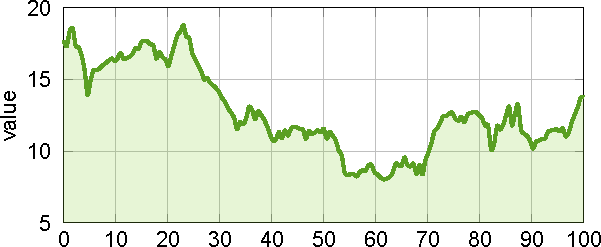
\includegraphics[width=0.7\textwidth]{Images/DivideAndConquer/shares-graph.pdf}
    \end{adjustbox}
    \caption{Stock value over time}
    \label{fig:divide_and_conquer:shares_value}
  \end{figure}
\end{frame}

%-------------------------------------------------------------------------------

\codeslide{python}{
  \begin{frame}{Divide and Conquer}{Example - Maximum Subtotal - Python}
    \textbf{Naive solution (brute force)}
    \onslide<2->
      \vspace{-0.5em}
      \lstinputlisting[
        language=Python,
        basicstyle=\small,
        tabsize=4,
        style={python-idle-code},
        escapechar={@},
        emph={maxSubArray},
        emphstyle=\color{blue}
      ]{Code/DivideAndConquer/MaxSubTotal_Naive.py}
    \end{frame}

    %-------------------------------------------------------------------------------

    \begin{frame}{Divide and Conquer}{Example - Maximum Subtotal - Python}
      \textbf{Runtime - Upper bound}
      \onslide<2->
      \vspace{-0.5em}
      \lstinputlisting[
        language=Python,
        basicstyle=\small,
        tabsize=4,
        style={python-idle-code},
        escapechar={@},
        emph={maxSubArray},
        emphstyle=\color{blue}
      ]{Code/DivideAndConquer/MaxSubTotal_Naive_Runtime.py}
    \end{frame}
}

%TODO: Implement for Java / C++

%-------------------------------------------------------------------------------

\begin{frame}{Divide and Conquer}{Example - Maximum Subtotal}
  \textbf{Upper bound:}
  \begin{itemize}
    \item<2->
      Three interleaved loops
    \item<3->
      Each loop with runtime {\color{Mittel-Blau}$O(n)$}
    \item<4->
      Algorithm runtime of {\color{Mittel-Blau}$O(n^3)$}
  \end{itemize}
\end{frame}

%-------------------------------------------------------------------------------

\begin{frame}{Divide and Conquer}{Example - Maximum Subtotal - Runtime}
  \textbf{Lower bound:}
  \begin{table}
    \caption{Operations}
    \label{fig:divide_and_conquer:max_sub_total_operations}
    \begin{tabular}{c|c|c}
      $i$ & Additions & $j$\\
      \midrule
      $\frac{n}{3} \in O(n)$ &
      $\frac{n}{3} \in O(n)$ &
      $\frac{n}{3} \in O(n)$\\
    \end{tabular}
  \end{table}
  \begin{itemize}
    \item<2->
      We iterate at least {\color{Mittel-Blau}$\frac{n}{3}$} values for {\color{Mittel-Blau}$i$}
    \item<3->
      For each {\color{Mittel-Blau}$i$} we iterate at least {\color{Mittel-Blau}$\frac{n}{3}$} values for {\color{Mittel-Blau}$j$}
    \item<4->
      For each {\color{Mittel-Blau}$j$} we have at least {\color{Mittel-Blau}$\frac{n}{3}$} additions
    \item<5->
      We need at least {\color{Mittel-Blau}$T(n) = (\frac{n}{3})^3 \in \Omega(n^3)$} steps
  \end{itemize}
  
\end{frame}

%-------------------------------------------------------------------------------

\begin{frame}{Divide and Conquer}{Example - Maximum Subtotal - Runtime}
  \textbf{Runtime:}
  \begin{itemize}
    \item<2->
      With {\color{Mittel-Blau}$T(n) \in O(n^3)$} and
      $T(n) \in {\color{Mittel-Blau}\Omega(n^3)}$ we know:
      \begin{displaymath}
        \color{Mittel-Blau}
        T(n) \in \Theta(n^3)
      \end{displaymath}
    \item<3->
      It is hard to solve the problem in a worse way $\ldots$
  \end{itemize}
\end{frame}

%-------------------------------------------------------------------------------

\begin{frame}{Divide and Conquer}{Example - Maximum Subtotal - Runtime}
  \textbf{Current approach:}
  \begin{itemize}
    \item<2->
      Calculating the sum for range from $i$ to $j$ with loop
      \begin{displaymath}
        S_{i,\,j} = X[i] + X[i+1] + \dots + X[j]
      \end{displaymath}
  \end{itemize}
  \onslide<3->
   \textbf{Better approach:}
   \begin{itemize}
    \item<4->
      Incremental sum instead of loop
      \begin{eqnarray*}
        S_{i,\,j+1} &=& X[i] + X[i+1] + \dots + X[j] + X[j+1]\\
        S_{i,\,j+1} &=& S_{i,\,j} + X[j+1]
        ~{\color{Mittel-Blau}\in O(1)}\hspace{1em} \text{instead of}\hspace{1em} {\color{Mittel-Blau}\in O(n)}
      \end{eqnarray*}
  \end{itemize}
\end{frame}

%-------------------------------------------------------------------------------

\codeslide{python}{
  \begin{frame}{Divide and Conquer}{Example - Maximum Subtotal - Python}
     \textbf{Better solution:}
     \onslide<2->
  \vspace{-0.5em}
  \lstinputlisting[
    language=Python,
    basicstyle=\small,
    tabsize=4,
    style={python-idle-code},
    escapechar={@},
    emph={maxSubArray},
    emphstyle=\color{blue}
  ]{Code/DivideAndConquer/MaxSubTotal.py}
   \begin{itemize}
   \item<3->Runtime {\color{Mittel-Blau}$\in O(n^2)$}
   \end{itemize}  
\end{frame}
}

%TODO: Implement for Java / C++

%-------------------------------------------------------------------------------

\begin{frame}{Divide and Conquer}{Example - Maximum Subtotal}
  \textbf{Divide and Conquer:}
  \vspace{-0.5em}
  \begin{figure}
    \begin{adjustbox}{width=\linewidth}
      \begin{tikzpicture}[
  list/.style={
    draw=black
  }, sum/.style={
    list,
    fill=Hell-Gruen
  }, label_sum/.style={
    color=black,
    font=\huge
  }
]%
% upper list
\draw[list] (0, 0) rectangle ++(16, 1);

\draw[sum] (1.5, 0) rectangle ++(2, 1);
\draw[sum] (6, 0) rectangle ++(5, 1);
\draw[sum] (13, 0) rectangle ++(2.5, 1);

\node[label_sum, anchor=south] at (2.5, 0) {A};
\node[label_sum, anchor=south] at (14.25, 0) {B};
\node[label_sum, anchor=south] at (7, 0) {rmax};
\node[label_sum, anchor=south] at (9.5, 0) {lmax};

\draw[list] (8, 1.5) -- (8, -0.5);

\draw[
  decorate,
  decoration={brace, raise=0.25em, amplitude=0.5em},
  thick
] (6, 1) -- node[midway, yshift=2em, label_sum] {C} (11, 1);
\end{tikzpicture}
    \end{adjustbox}
    \label{fig:divide_and_conquer:max_sub_total_divide}
  \end{figure}
   \vspace{-0.5em}
  \begin{itemize}
  \item<2->
    Solve the left / right half of the problem
  \item<3->
    Combine both solutions into a total solution
  \item<4->
    The maximum is located in the {\color{Mittel-Blau}left~half~($A$)}
    or the {\color{Mittel-Blau}right~half~($B$)}
  \item<5->
    The maximum can {\color{Mittel-Blau}extend into the second half ($C$)}
  \item<6->
    To solve $C$ we have to calculate $rmax$ and $lmax$
  \item<7->
    The overall solution is the {\color{Mittel-Blau}maximum of $A$, $B$ and $C$}
  \end{itemize}
\end{frame}

%-------------------------------------------------------------------------------

\begin{frame}{Divide and Conquer}{Example - Maximum Subtotal}
  \textbf{Principle - Divide and Conquer:}
  \begin{itemize}
    \item<2->
      Small problems are solved directly: {\color{Mittel-Blau}$n = 1 \Rightarrow \max = X[0]$}
    \item<3->
      Bigger problems are partitioned into two subproblems and recursivly solved. Subsolutions A and B
      are returned.
    \item<4>
      To determine subsolution C, rmax and lmax for the subproblems are computed.
    \item<5>
      The overall solution is the {\color{Mittel-Blau}maximum of $A$, $B$ and $C$}
  \end{itemize}
\end{frame}

%-------------------------------------------------------------------------------


\codeslide{python}{
  \begin{frame}{Divide and Conquer}{Example - Maximum Subtotal - Python}
  \textbf{Divide and conquer solution} 
  \vspace{-0.5em}
  \lstinputlisting[
    language=Python,
    basicstyle=\small,
    tabsize=4,
    style={python-idle-code},
    escapechar={@},
    emph={maxSubArray},
    emphstyle=\color{blue}
  ]{Code/DivideAndConquer/MaxSubTotal_DivideAndConquer.py}
\end{frame}
}

%TODO: Implement for Java / C++
